\PassOptionsToPackage{full}{textcomp}
\documentclass[]{tufte-handout}
%\usepackage{fontspec}

% load babel package and options here
%\usepackage[p,osf]{ETbb} % osf in text, tabular lining figures in math
\usepackage{ETbb} % osf in text, tabular lining figures in math
\usepackage[scaled=.95,type1]{cabin} % sans serif in style of Gill Sans
\usepackage[varqu,varl]{zi4}% inconsolata typewriter
\usepackage[T1]{fontenc} % LY1 also works
\usepackage[libertine,vvarbb]{newtxmath}
%\usepackage[cal=boondoxo,bb=boondox,frak=boondox]{mathalfa}

%\geometry{showframe} % display margins for debugging page layout

\usepackage{graphicx} % allow embedded images
%  \setkeys{Gin}{width=\linewidth,totalheight=\textheight,keepaspectratio}
  \graphicspath{{graphics/}} % set of paths to search for images
\usepackage{amsmath}  % extended mathematics
\usepackage{booktabs} % book-quality tables
%\usepackage{units}    % non-stacked fractions and better unit spacing
\usepackage{multicol} % multiple column layout facilities
\usepackage{lipsum}   % filler text
\usepackage{fancyvrb} % extended verbatim environments
  \fvset{fontsize=\normalsize}% default font size for fancy-verbatim environments
\usepackage{gensymb} % provides symbols like \degree
\usepackage{ragged2e} % enables hyphenation in ragged-right justification
\usepackage[normalize-symbols]{textalpha} %enables \textalpha for alpha symbol etc.

\usepackage{hyperref} % enables styling of href and url
\hypersetup{
    pdftitle={Mechanisms},
    pdfauthor={Barry Linkletter},
    colorlinks=true,
    linkcolor=blue,
    filecolor=magenta,      
    urlcolor=blue,
    pdfborder={0 0 0},
    frenchlinks=false,
    pdfpagemode=FullScreen,
    }
    \urlstyle{same}
\makeatletter
% Inspired by http://anti.teamidiot.de/nei/2009/09/latex_url_slash_spacingkerning/
% but slightly less kern and shorter underscore
\let\UrlSpecialsOld\UrlSpecials
\def\UrlSpecials{\UrlSpecialsOld\do\/{\Url@slash}\do\_{\Url@underscore}}%
\def\Url@slash{\@ifnextchar/{\kern-.03em\mathchar47\kern-.15em}%
    {\kern-.0em\mathchar47\kern-.08em\penalty\UrlBigBreakPenalty}}
\def\Url@underscore{\nfss@text{\leavevmode \kern.06em\vbox{\hrule\@width.3em}}}
\makeatother

\usepackage{enumitem} % allows resuming enumerate lists.
\usepackage{mathtools}
\usepackage{mhchem}

\usepackage{siunitx} % provides "S" column class for aligning decimals.  
         \sisetup{uncertainty-mode = separate}

\usepackage{nicefrac}

\usepackage[nospace]{varioref}
    \renewcommand\reftextfaceafter{on the following page}
    \renewcommand\reftextafter {on the next page}
    \renewcommand\reftextfacebefore{on the previous page}
    \renewcommand\reftextbefore {on the previous page}

\newcommand{\tss}[1]{\textsuperscript{#1}}

\usepackage[english]{babel}
\usepackage{float}
\usepackage{stackrel}

\usepackage[shortconst]{physconst}

\usepackage[normalem]{ulem}  % provides strikethrough \sout{}

\usepackage{newfloat}
\DeclareFloatingEnvironment[
  fileext = los ,
  listname = {List of Schemes} ,
  name = Scheme
]{scheme}

\usepackage{newfloat}
\DeclareFloatingEnvironment[
  fileext = loe ,
  listname = {List of Eqs} ,
  name = Equation
]{equate}

\usepackage{listings}

%%%%%%%%%%%%%%%%%%%%%%%%%%%%%%%%%%%%%%%%%%%%%%%%%%%%%%%%%%%


\title{Extreme Ester Hydrolysis}
\author[Barry Linkletter]{Barry Linkletter}
\date{} % without \date command, current date is supplied


\begin{document}

\justifying
\maketitle
\marginnote[-15mm]{This document was produced using the \LaTeX\ typesetting language with the Tufte-handout document class. Chemical diagrams were created in \textit{ChemDoodle} and calculations and plotting were performed using \textit{Python} tools in a \textit{Jupyter Notebook}. Diagrams and plots were further edited in \textit{Affinity Designer}\vspace{3mm}}

\begin{abstract}

\noindent This exploration consider acid-catalyzed hydrolysis of esters in extreme acid conditions.

\end{abstract}





\section{Possible Mechanisms for Hydrolysis}

Let us consider the possible mechanisms for hydrolysis of esters in extreme acid media. We will be using data from a Canadian contribution that reports rates of ester hydrolysis in mixtures of sulphuric acid and water.\sidenote[][-10mm]
{"Mechanisms of ester hydrolysis in aqueous sulfuric acids."
K. Yates, R.A. McClelland,
\textit{J. Am. Chem. Soc.}, \textbf{1967}, \textit{89}, 2686-2692.
\url{https://doi.org/10.1021/ja00987a033} \label{ref:ref1}}

Ester hydrolysis in acid can occur via an acid-catalyzed mechanism that involves activation of the carbonyl group by equilibrium protonation, followed by a rate-determining addition reaction. This is designated as an $\rm A_{Ac}2$ mechanism. However, is some cases, there are other observed mechanisms.


\begin{figure*}[h!]
  \centering
  \caption[][-0mm]{Acid-catalyzed hydrolysis of an ester via a bimolecular acyl substitution reaction ($\rm A_{Ac}2$). $\uparrow$} 
  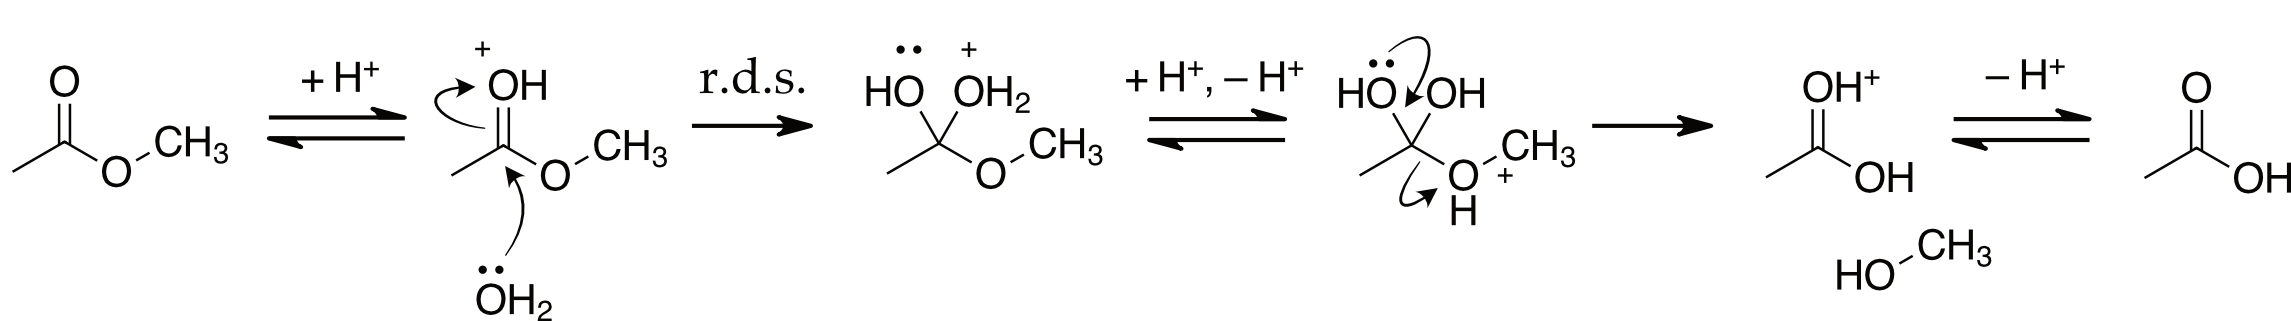
\includegraphics[scale=0.7]{images/AAc2}
  \label{fig:fig1}
\end{figure*}

If the substituent on the carbonyl group can stabilize a carbocation then it is possible that the fastest route to hydrolysis would be via the unimolecular departure of the protonated alcohol group. This is designated as an $\rm A_{Ac}1$ mechanism. The acylium ion intermediate is generally only observed when the substituent is stabilizing and the conditions have minimal nucleophiles present. Mixtures that are mostly \ce{H2SO4} will have very little free water available to act as a nucleophile. Perhaps we will see this mechanism become important in extreme acid mixtures.

\begin{figure}[h!]
  \centering
  \caption[][-0mm]{Acid-catalyzed hydrolysis of an ester via a unimolecular departure of the leaving group ($\rm A_{Ac}1$).\\ $\longleftarrow$} 
  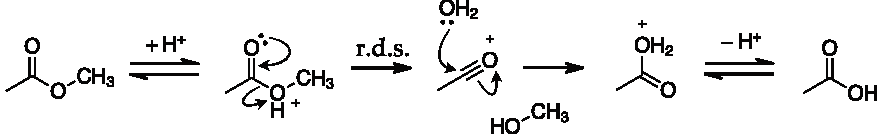
\includegraphics[scale=0.7]{images/AAc1}
  \label{fig:fig2}
\end{figure}

If the nucleophile cannot attack the carbonyl group for some reason (e.g. sterics) then we may see the hydrolysis occur via an $\rm S_N2$ substitution reaction at the carbon of the alcohol group. This is designated as an $\rm A_{Al}2$ mechanism.

\begin{figure}[h!]
  \centering
  \caption[][-0mm]{Acid-catalyzed hydrolysis of an ester via nucleophilic attack at the carbon of the alcohol group ($\rm A_{Al}2$).\\ $\longleftarrow$} 
  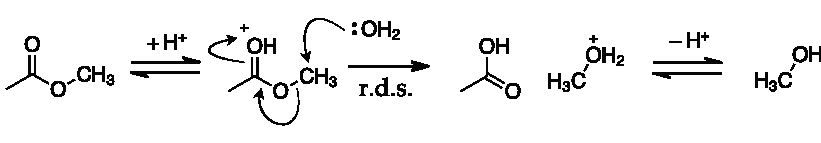
\includegraphics[scale=0.7]{images/AAl2}
  \label{fig:fig3}
\end{figure}

If the carbon of the alcohol group in the ester can bear a positive charge easily then we may see a unimolecular dissociation of the acid group from that carbon to give a carbocation. The \emph{t}-butyl group is a classic example and it has a famous abbreviation -- Boc. Other carbon groups may also result in this mechanism becoming predominant in minimally nucleophilic conditions such as extreme acid mixtures. This is an example of an $\rm A_{Al}1$ mechanism.

\begin{figure}[h!]
  \centering
  \caption[][-0mm]{Acid-catalyzed hydrolysis of an ester via dissociation of the carbon of the alcohol group ($\rm A_{Al}1$).\\ $\longleftarrow$} 
  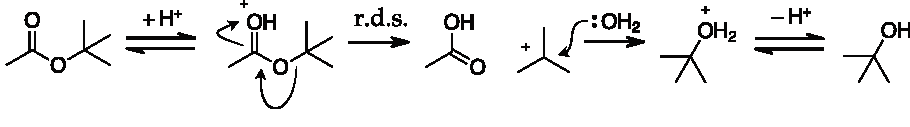
\includegraphics[scale=0.7]{images/AAl1}
  \label{fig:fig4}
\end{figure}

The $\rm A_{Ac}$ and $\rm A_{Al}$ mechanisms can be distinguished by isotopic labeling of water, by secondary kinetic isotope effects or by observing the stereochemistry of the alcohol product. The unimolecular and bimolecular mechanisms can be distinguished by observing a rate dependance on the activity of water. The Yates paper\textsuperscript{\ref{ref:ref1}} investigates the kinetics for hydrolysis of several esters in acid mixtures with a wide range of water activity. All four of the above reaction pathways are observed, depending on the ester and the reaction conditions.


\subsection{The $\rm A_{Ac}2$ Mechanism}

On examination of the $\rm A_{Ac}2$ mechanism presented in figure~\ref{fig:fig1} above, we can establish the reaction scheme and rate law.\vspace{-5mm}
\begin{scheme}[h!]
  \caption[][5mm]{Reaction scheme for the $\rm A_{Ac}2$ mechanism. `S' is the ester substrate for the reaction. \\ $\longleftarrow$} 
  \label{sch:sch1}
  \begin{align*} 
    \ce{S + H^+ &<=>[][$K_a$] SH^+} \\
    \ce{SH^+ + n H2O  &->[$k$] P}
  \end{align*}
\end{scheme}

The rate law can be expressed as shown in eq.~\ref{eq:1} below. Take note of the stoichiometry term, $n$, for water. Yates et al. were investigating the possibility of a higher-order dependance on \ce{[H2O]} in highly acidic media. In dilute water it is impossible to determine how many waters are involved in the transition state for the rate-determining addition step. This is unimportant as the concentration of water in dilute solution does not change and it is folded into the pseudo-first order rate constant for the reaction. But what if the concentration of water was actually changing?

\begin{equation}
   \frac{\partial}{\partial t} P =  k\frac{[\ce{H+}]}{K_a + [\ce{H+}]}[\ce{H2O}]^n \cdot [\ce{S}]_t
  \label{eq:1}
\end{equation}

%\newpage
The pseudo-first order rate constant can be defined as\ldots

\begin{equation}
   k_{obs} =  k\frac{[\ce{H+}]}{K_a + [\ce{H+}]}[\ce{H2O}]^n \textrm{ where } \frac{\partial}{\partial t} [\ce{P}] =  k_{obs}\cdot [\ce{S}]_t
  \label{eq:2}
\end{equation}

Of course, we are well beyond a dilute solution where ideal behaviour of ions is assumed. We should use the activities of acid and water, not their actual concentrations. The activity of acid can be expressed using an acidity function such as $H_0$. 
\begin{equation}
   H_0 = -\log{h_0}
  \label{eq:3}
\end{equation}

\vspace{0mm}

\begin{marginfigure}[-5mm]
  \centering
  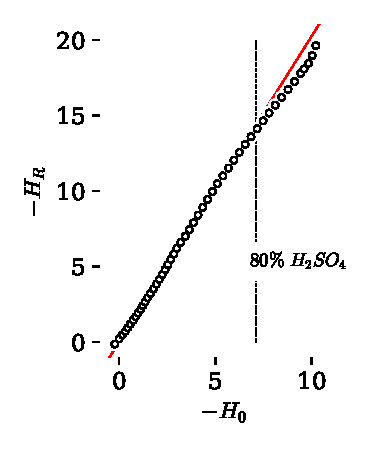
\includegraphics[scale=0.7]{images/H0HrCorrelation}
  \caption{A plot of $H_R$ vs. $H_0$. $\uparrow$ \\ \vspace{1mm} It is a linear trend, although imperfect. We observe that $H_R \approx 1.95H_0$ in the range of 4 to 80\%. Compare with figure~2 in the Yates paper\textsuperscript{\ref{ref:ref1}} The \textit{Python} notebook for this plot can accessed via Google Colab at \url{https://colab.research.google.com/github/blinkletter/4410PythonNotebooks/blob/main/Class_30/Yates-Fig5-HRH0.ipynb}\vspace{5mm}} 
  \label{fig:fig5}
\end{marginfigure}


$h_0$ is the activity of the acidic medium for transferring a proton to the aniline nitrogen of an indicator dye. The aniline system behaves differently than an ester for protonation. Due to their reactivity, there have been no acidity functions for ester substrates reported. The authors measured the protonation of some unreactive esters in high concentrations of \ce{H2SO4} and determined an acidity function for esters, $H_S = 0.62 H_0$, They made the assumption that this relationship would hold true across the range of \ce{H2SO4} mixtures used. The fact that other acidity functions such as $H_R$ show a linear proportionality with $H_0$ backs up this assumption. I plotted literature data sets for $H_0$ and $H_R$ in figure~\ref{fig:fig5}. Do you agree?

The activity of water, $a_{\ce{H2O}}$ in various mixtures with \ce{H2SO4} can be measured. Tables for $a_{\ce{H2O}}$ are available in the literature.\sidenote[][0mm]{``The Thermodynamic Properties of Aqueous Sulfuric Acid Solutions and Hydrates from 15 to 300 K.''
W. F. Giauque, E. W. Hornung, J. E. Kunzler, and T. R. Rubin
\textit{J. Am. Chem. Soc.}, \textbf{1960}, \textit{82}, 62-70
\url{https://doi.org/10.1021/ja01486a014} \vspace{3mm} \label{ref:ref2}}
We can now state $k_{obs}$ in terms of $h_0$ and $a_{\ce{H2O}}$\ldots
\begin{equation}
   k_{obs} =  k\frac{h_0^m}{K_a^m + h_0^m}a_{\ce{H2O}}^n \textrm{,  where }m = 0.62
  \label{eq:4}
\end{equation}

We can now construct a log-log plot of the form\ldots\sidenote[][-0mm]{The authors assume that $h_0 \ll K_a$ and so the plot will collapse to the form presented in the paper\ldots
\begin{align*}
   \log{k_{obs}}+m H_0 &= n\log{a_{\ce{H2O}}} + (mp{K_a}+\log{k}) \\
  \log{k_{obs}}+m H_0 &= n\log{a_{\ce{H2O}}} + const.
  \label{eq:6}
\end{align*}

The approach that I am using here is mentioned in footnote~21 of the paper.\textsuperscript{\ref{ref:ref1}}
}

\begin{equation}
   \log{k_{obs}}-\log{\frac{h_0^m}{K_a^m + h_0^m}} =  n\log{a_{\ce{H2O}} + \log{k}} 
  \label{eq:5}
\end{equation}

\section{Reaction Kinetics for Methyl Acetate}

The rate data for methyl acetate (and several other esters) in mixtures of sulphuric acid is provided in the paper. The data is listed in table~\ref{tab:tab1} and the plots of $k_{obs}$ vs. \%\ce{H2SO4} and mole fraction \ce{H2SO4} ($X_{H_2SO_4}$) are presented in figure~\ref{fig:fig2}.


\begin{figure*}[h!]
  \centering
  \caption[][-0mm]{Plots of $k_{obs}$ vs. $\%\ce{H2SO4}$ and $k_{obs}$ vs mole fraction \ce{H2SO4}. $\uparrow$ \\ \vspace{1mm}The grey dashed line is the activity of water and the red dashed line is the mole fraction of water. Curves are Bspline interpolations of smoothed data. The \textit{Python} notebook for this plot can accessed via Google Colab at \url{https://colab.research.google.com/github/blinkletter/4410PythonNotebooks/blob/main/Class_30/Yates-Fig6-MeOAc.ipynb}\vspace{5mm}} 
  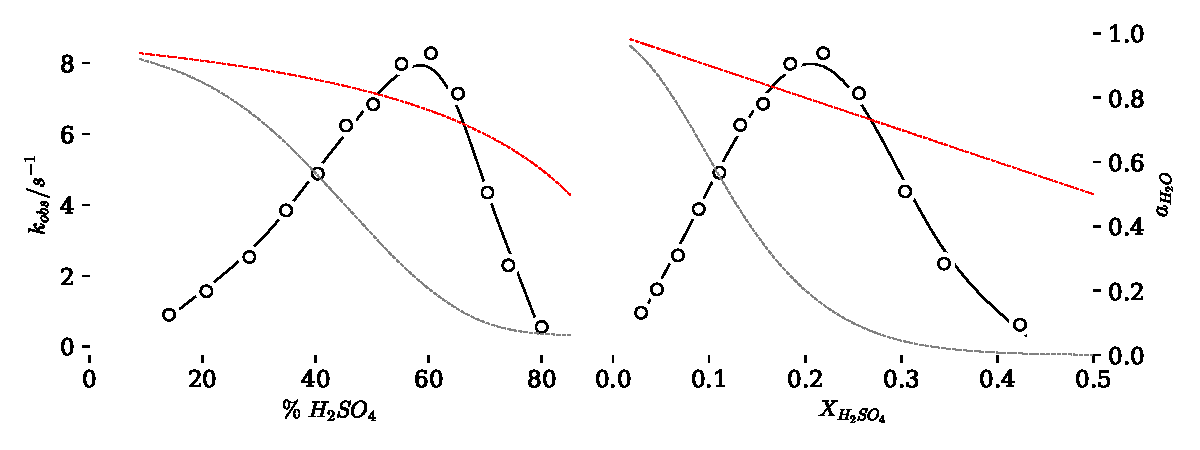
\includegraphics[scale=0.7]{images/fig2}
  \label{fig:fig6}
\end{figure*}

The lines in the plots are smoothed interpolations and do not represent any mathematical model. Observe that the rate increases as the amount of sulphuric acid in the mixture increases. However, as the acid content increases the rate eventually starts dropping. Examination of the rate law for the $\rm A_{Ac}2$ reaction shows that the rate is dependant on both acidity and the amount of water available to act as a nucleophile. The red dashed line on the plots is the mole fraction of water, $X_{H_2O}$. We see that the concentration of water diminishes in stronger acid mixtures, however this reduction in concentration is not enough to explain the drop in rate. What is really dropping is the activity of the water, $a_{H_2O}$, shown in the gray dashed line. The $a_{H_2O}$ is the apparent mole fraction of water in the mixture. It drops rapidly as we increase the amount of acid because hydronium ion is not a nucleophile.\sidenote[][-40mm]{Compare figure~\ref{fig:fig6} above with figure~1 in the paper.\tss{\ref{ref:ref1}} Note that the figure presented by Yates et al. shows a second mechanism becoming predominate at very high acidity. The data for these final few points is not included in Table~1 of their paper. This was likely a printing error. There was no erratum published so the authors obviously didn't feel that this omission was a big deal. We would not have used those final points anyway as they are the result of an alternate mechanism and do not represent the kinetics of the $A_{Ac}2$ pathway.}


\subsection{A Log-Log Plot}

A log-log plot would be better for interpreting the rate vs. acidity. We will use the acidity function, $-H_S$, to represent the log of the activity of acid. We will plot $\log{a_{H_2O}}$ against $-H_S$ as presented in figure~\ref{fig:fig7}.

\begin{figure}[h!]
  \centering
  \caption[][10mm]{Log-log plot of $k_{obs}$ and $a_{H_2O}$ vs. $H_S$. The grey dashed line is $\log{a_{H_2O}}$ and the red line is a simple slope of 1.0, representing theoretical first-order dependance on the acidity of the mixture. \\ $\longleftarrow$ \\ \vspace{1mm} Curves are Bspline interpolations of smoothed data. The \textit{Python} notebook for this plot can accessed via Google Colab at \url{https://colab.research.google.com/github/blinkletter/4410PythonNotebooks/blob/main/Class_30/Yates-Fig7-MeOAc.ipynb}} 
  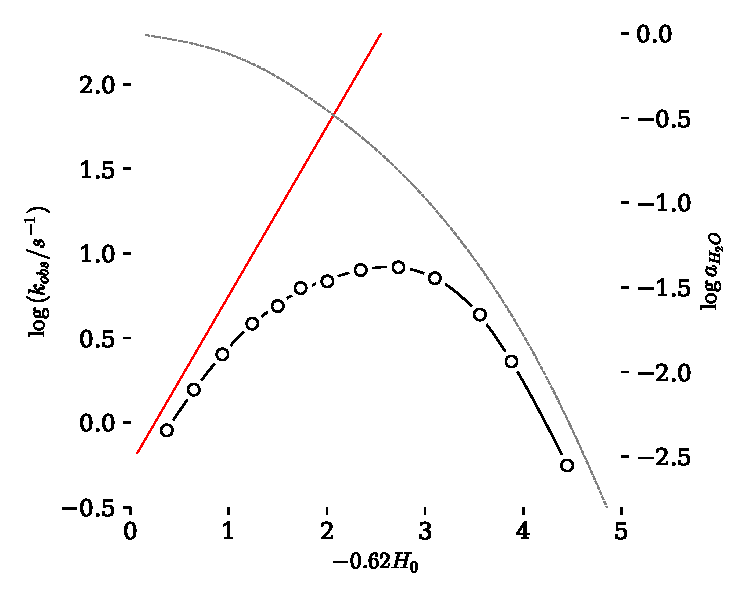
\includegraphics[scale=0.7]{images/fig3}
  \label{fig:fig7}
\end{figure}

\begin{margintable}[30mm]
\centering
\caption{Pseudo-first order rate constants for hydrolysis of methyl acetate at \qty{25}{\degreeCelsius}.\textsuperscript{\ref{ref:ref1}}$\downarrow$\vspace{3mm}}
\label{tab:tab1}
    \begin{tabular}{SS}
%        \toprule
        {$\%\ce{H2SO4}$}      & {$k_{obs}/\qty{e{-2}}{min^{-1}}$} \\
        \midrule
           14.1    &   1.50    \\
           20.7    &   2.61    \\
           28.3    &   4.22    \\
           34.8    &   6.41    \\
           40.4    &   8.14    \\
           45.4    &  10.4     \\
           50.2    &  11.4     \\
           55.2    &  13.3     \\
           60.4    &  13.8     \\
           65.2    &  11.9     \\
           70.4    &   7.25    \\
           74.1    &   3.83    \\
           80.0    &   0.931   \\
%        \bottomrule
    \end{tabular}
\end{margintable}

According to the rate law, the log-log plot should have a slope of 1 in acidic conditions and then curve over to a slope of zero when the system is more acidic than the $pK_a$ of the protonated ester and $[\ce{SH+}]$ approaches a maximum value. We do see that the slope of the curve seems to approach 1.0 as the solution becomes more dilute. However, we do not observe the rate reaching a constant value, rather it decreases sharply as the mole fraction of \ce{H2SO4} increases. As discussed above, this is because the value of $k_{obs}$ is also dependant on the activity of water, $a_{\ce{H2O}}$.

\subsection{Plotting the Rate Law}

The rate law established in equation~\ref{eq:5} above would allow us to plot the rate (as dependant on $H_S$) against $a_{H_2O}$. We should obtain a straight line with a slope equal to the molecularity (reaction order) of water. Yates et al. were investigating the observation that these ester hydrolysis reactions involved multiple water molecules in the transition state of the r.d.s. and so we should be prepared to see the slope be greater than one.

However, we will first replicate the exact approach of the authors where they assume that the fraction of $\nicefrac{\ce{SH+}}{\ce{S}}$ is minimal ($H_0<pK_a$). The authors plotted the following relationship shown in equation~\ref{eq:6} and the plot is presented in figure~\ref{fig:fig8} below.

\begin{align}
  \log{k_{obs}}+m H_0 &= n\log{a_{\ce{H2O}}} + const.
  \label{eq:6}
\end{align}

We observe the same results as reported by the authors: $n = 1.92$. We see from the rate law in equation~\ref{eq:1} that $n$ is the order in \ce{H2O}.

\marginnote[-20mm]{The \textit{Python} notebook for the plots in Figures~\ref{fig:fig8} and \ref{fig:fig9} below can accessed via Google Colab at \url{https://colab.research.google.com/github/blinkletter/4410PythonNotebooks/blob/main/Class_30/Yates-Fig8-rate_vs_aH2O.ipynb}}

\begin{figure}[h!]
  \centering
  \caption[][-0mm]{Plot of $\log{k_{obs}}+m H_0$ vs. $\log{a_{\ce{H2O}}}$. $m$ is set to 0.62. Compare this plot to figure~3 of the paper.\textsuperscript{1}\\ $\longleftarrow$ \\ The line equation is\ldots 
  \begin{align*}
  y &= 1.92x-0.31 \\ 
  r^2 &= 0.999
  \end{align*}} 
  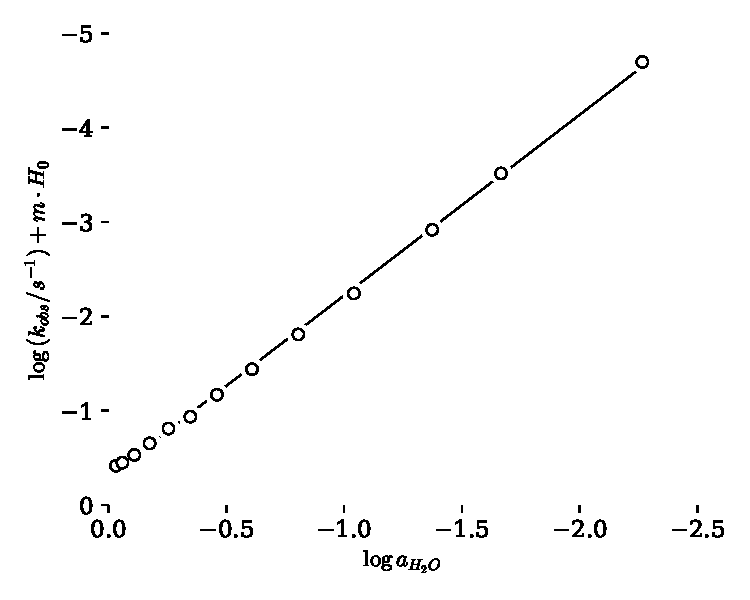
\includegraphics[scale=0.7]{images/fig8}
  \label{fig:fig8}
\end{figure}


\begin{marginfigure}[-15mm]
  \centering
  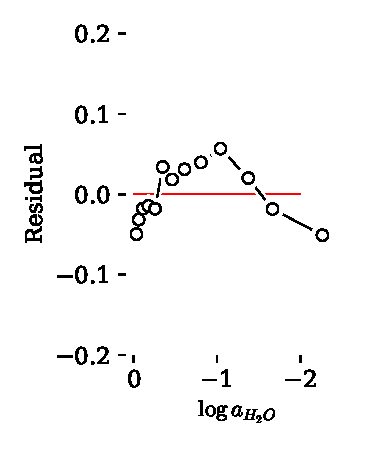
\includegraphics[scale=0.7]{images/fig8r}
  \caption{A plot of the residuals. $\uparrow$} 
  \label{fig:fig9}
\end{marginfigure}

We would conclude that the rate-determining-step involves two molecules of water and this idea is discussed at length in the paper.\textsuperscript{\ref{ref:ref1}} I challenge you to apply this plotting method to the other ester results presented in the paper and you should see the same results for the data describing the $A_{Ac}2$ mechanism. Compare your results to those reported in table~II of the paper.
\newpage
\section{Comments and Criticisms}

As always, I have some notes. Observe the plot of the residuals for figure~\vref{fig:fig8} presented in figure~\ref{fig:fig9}. The line fit is excellent ($r^2 = 0.999$) and the deviation from the line fit is small, but we observe a systematic pattern in the residual plot. We are not capturing the full system in our model.

\begin{marginfigure}[-0mm]
  \centering
  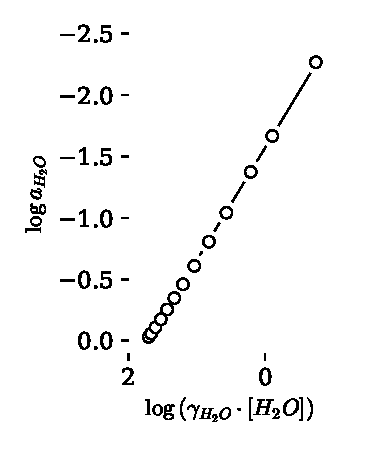
\includegraphics[scale=0.7]{images/fig12}
  \caption{  \label{fig:fig12}
A log-log plot of $a_{\ce{H2O}}$ vs. $\gamma_{\ce{H2O}} \cdot [\ce{H2O}]$. $\uparrow$  The line equation is\ldots 
\begin{align*}
y &= 0.92x-1.57 \\  
r^2 &= 0.9998
\end{align*}} 
\end{marginfigure}

The values of $a_{\ce{H2O}}$ used by the authors are clearly not in units of molar concentration. Upon examination of the data in the referenced publication,\textsuperscript{\ref{ref:ref2}} we see that $a_{\ce{H2O}}$ is the ``apparent mole fraction'' of water in the mixture, $\gamma_{\ce{H2O}} \cdot X_{\ce{H2O}}$ and not the effective concentration of water, $\gamma_{\ce{H2O}} \cdot [\ce{H2O}]$. 


We can calculate $\gamma_{\ce{H2O}}$ using the data table\textsuperscript{\ref{ref:ref2}} of $a_{\ce{H2O}}$ vs. $\%\ce{H2SO4}$ and we can obtain $[\ce{H2O}]$ vs. $\%\ce{H2SO4}$ from literature data tables.\sidenote
[][5mm]{"CRC Handbook of Chemistry and Physics." Many copies are available in the library stacks (QD65.H3) and there is an \href{https://library.upei.ca/chem}{online version available}. A data table that lists the \href{https://hbcp-chemnetbase-com.proxy.library.upei.ca/documents/05_29/05_29_0084.xhtml?dswid=7040}{densities of mixtures of sulfuric acid} can be found on page 9-84 of the 2025 edition.}

 With a little effort we can convert $a_{\ce{H2O}}$ to $\gamma_{\ce{H2O}} \cdot [\ce{H2O}]$. Plotting the two sets of values against each other shows that they are similar as presented in figure~\ref{fig:fig12} where we see a linear relationship with a slope near unity. So all this work won't change the result much, but it will make it more defensible.

\begin{figure}[h!]
  \centering
  \caption[][20mm]{Plot of $\log{k_{obs}}+m H_0$ vs. $\gamma_{\ce{H2O}} \cdot [\ce{H2O}]$.\\ $\longleftarrow$ \\ The line equation is\ldots \begin{align*}y &= 1.75x-0.33 \\ r^2 &= 0.998\end{align*}} 
  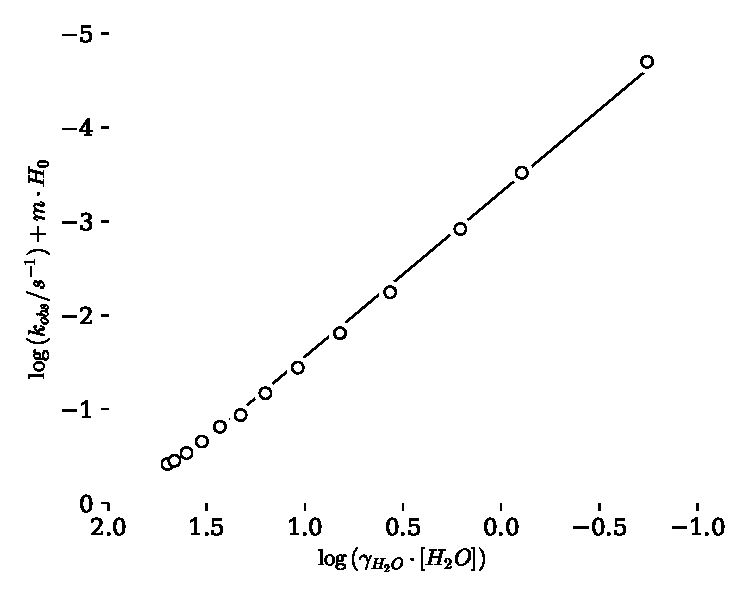
\includegraphics[scale=0.7]{images/fig10}
  \label{fig:fig10}
\end{figure}


\begin{marginfigure}[35mm]
  \centering
  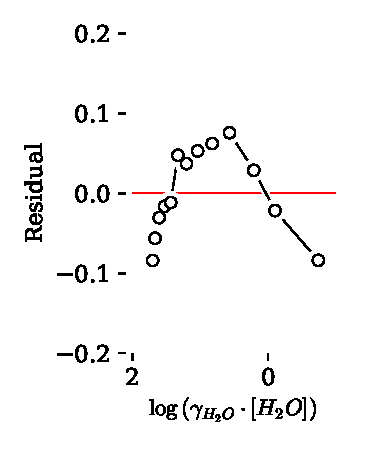
\includegraphics[scale=0.7]{images/fig10r}
  \caption{A plot of the residuals. $\uparrow$ \\ \vspace{3mm} The \textit{Python} notebook for the plots in Figures~\ref{fig:fig12}, \ref{fig:fig10} and \ref{fig:fig11} above can accessed via Google Colab at \url{https://colab.research.google.com/github/blinkletter/4410PythonNotebooks/blob/main/Class_30/Yates-Fig10-rate_vs_gammaH2O.ipynb}} 
  \label{fig:fig11}
\end{marginfigure}

Again we get a great correlation but still see the systematic variation in the residuals that indicates an incomplete model.

\subsection{Including the $K_a$ Value}

The authors used a rate law that assumed the magnitude of the acidity was well below the $pK_a$ ($H_0<pK_a$). This is almost true, but in the data we will see that $H_0$ is approaching the value of $pK_a$ and, for some of the data points, there could be deviation from the model.

To account for this we should plot the full rate law as described in equation~\vref{eq:5}. We will need a value for the $pK_a$ of the \ce{SH+} species (the protonated ester). The authors quote a value of $-7.2$ and that is what we will use for now.\sidenote[][0mm]{``The possibility of a cyclic mechanism for acid-catalyzed ester hydrolysis.''
C.A. Lane, M.F. Cheung, and G.F. Dorsey,
\textit{J. Am. Chem. Soc.}, \textbf{1968}, \textit{90}, 6492-6494.
\url{https://doi.org/10.1021/ja01025a046} \label{ref:ref6}} The authors also defined the $H_S$ scale as $H_s = m\cdot H_0$ and measured the value of $m$ to be $0.62$ based on spectroscopic observations of ester protonation.\textsuperscript{\ref{ref:ref1}} Based on these parameters we can create a model for the rate law from equation~\ref{eq:5} (reproduced below, with the values of $m$ and $K_a$ stated.) 

\begin{align*}
   \log{k_{obs}}-\log{\frac{h_0^m}{K_a^m + h_0^m}} &=  n\log{a_{\ce{H2O}} + \log{k}} \\
   m &= 0.62 \\
   K_a &= 10^{7.2} \\
   a_{\ce{H2O}} &= \gamma_{\ce{H2O}} \cdot [\ce{H2O}]
  \label{eq:5X}
\end{align*}

Let us plot $\log{k_{obs}}-\log{\frac{h_0^m}{K_a^m + h_0^m}}$ vs. $\gamma_{\ce{H2O}} \cdot [\ce{H2O}]$ as presented in figure~\ref{fig:fig13} using the values for $m$ and $pK_a$ selected by Yates et al.

\begin{figure}[h!]
  \centering
  \caption[][-0mm]{Plot of $\log{k_{obs}}-\log{\frac{h_0^m}{K_a^m + h_0^m}}$ vs. $\gamma_{\ce{H2O}} \cdot [\ce{H2O}]$ where $m = 0.62$ and $pK_a = -7.2$.\\ $\longleftarrow$ \\ The line equation is\ldots \begin{align*}y &= 1.66x+1.28 \\ r^2 &= 0.999\end{align*}} 
  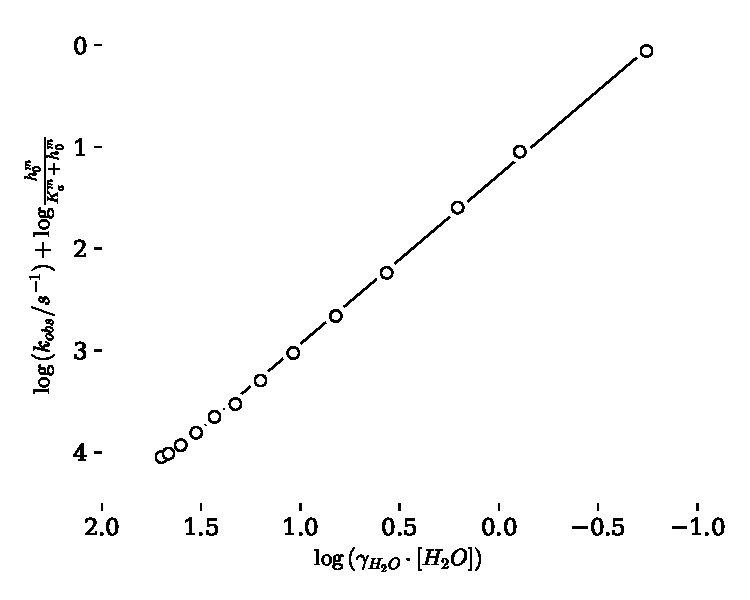
\includegraphics[scale=0.7]{images/fig13}
  \label{fig:fig13}
\end{figure}


\begin{marginfigure}[10mm]
  \centering
  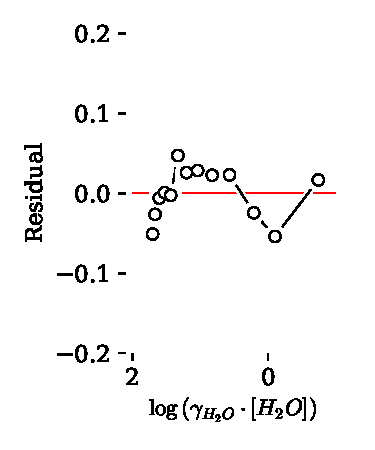
\includegraphics[scale=0.7]{images/fig13r}
  \caption{A plot of the residuals. $\uparrow$  \\ \vspace{3mm} The \textit{Python} notebook for the plots in Figures~\ref{fig:fig13} and \ref{fig:fig14} above can accessed via Google Colab at \url{https://colab.research.google.com/github/blinkletter/4410PythonNotebooks/blob/main/Class_30/Yates-Fig13-rate_vs_gammaH2O.ipynb}} 
  \label{fig:fig14}
\end{marginfigure}

Again we have a plot with an amazing correlation coefficient and a set of residuals that follows the line fit closely. There still seems to be structure to the residual plot that is beyond random variation but it is now much less pronounced. The slope is about 1.7, which still is indicative of more than one water molecule being involved in the r.d.s. We shall soon see that the slope is very sensitive to the value of $m$ that we choose. This may also be due to a lack of an accurate acidity function for ester protonation in extreme acid conditions. Recall that the authors ball-parked their tentative $H_S$ scale by setting it as a fraction of $H_0$ ($H_S = 0.62H_0$.)
\clearpage
\subsection{Optimizing the Values for $m$ and $pK_a$}

We now know that the line fit is dependant on the set values of $m$ and $pK_a$. Changing these constants will change the values on the Y-axis and affect the slope and the quality of the fit. So far, our line fits have been fantastic no matter what we do. Will that hold up if we tweak the constants that define the behaviour of the ester acid equilibrium?

\begin{marginfigure}[-0mm]
  \centering
  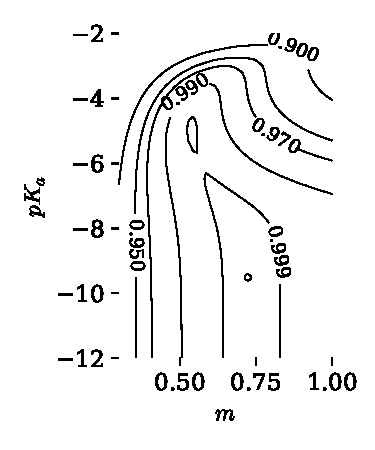
\includegraphics[scale=0.7]{images/fig15}
  \caption{A contour plot of the surface for $r^2$ as $m$ and $pK_a$ are surveyed. the best fit occurs at $m = 0.72$ and $pK_a = -9.5$ although the surface is very flat for a broad area around those values. $\uparrow$} 
  \label{fig:fig15}
\end{marginfigure}


I will survey a series of values for $m$ and $pK_a$ and determine the value of the Pearson correlation constant, $r^2$ for the line fit of $\log{k_{obs}}-\log{\frac{h_0^m}{K_a^m + h_0^m}}$ vs. $\gamma_{\ce{H2O}} \cdot [\ce{H2O}]$ in each case. Figure~\ref{fig:fig15} shows a contour plot that explores the surface for $r^2$ w.r.t. these two constants. Optimizing for the fit gives a values of $m = 0.72$ and $pK_a = -9.5$. 

\begin{figure}[h!]
  \centering
  \caption[][20mm]{Plot of $\log{k_{obs}}-\log{\frac{h_0^m}{K_a^m + h_0^m}}$ vs. $\gamma_{\ce{H2O}} \cdot [\ce{H2O}]$ where $m = 0.72$ and $pK_a = -9.5$. \\ $\longleftarrow$ \\ The line equation is\ldots \begin{align*}y &= 2.01x+2.93 \\ r^2 &= 0.999\end{align*}} 
  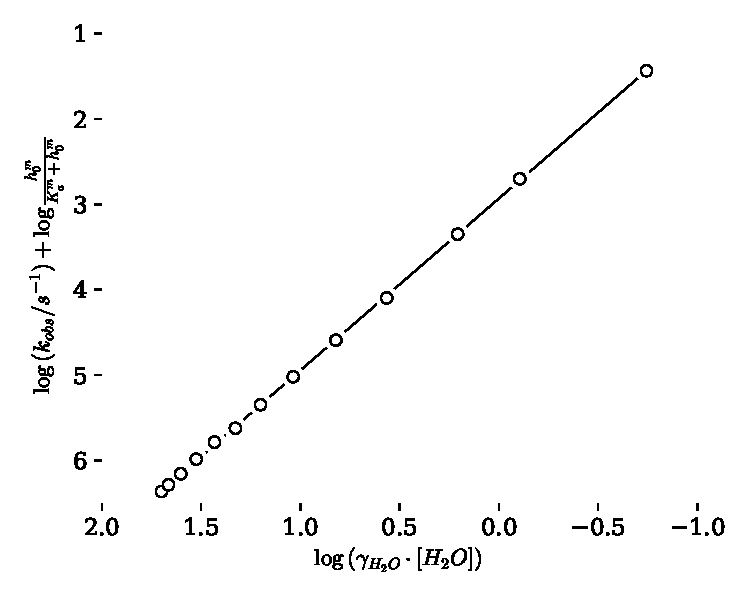
\includegraphics[scale=0.7]{images/fig16}
  \label{fig:fig16}
\end{figure}


\begin{marginfigure}[45mm]
  \centering
  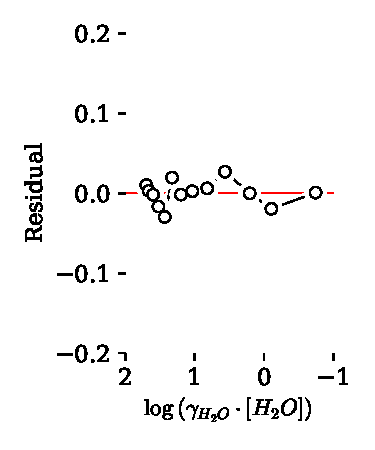
\includegraphics[scale=0.7]{images/fig16r}
  \caption{A plot of the residuals. $\uparrow$  \\ \vspace{3mm} The \textit{Python} notebook for the plots in Figures~\ref{fig:fig15}, \ref{fig:fig16} and \ref{fig:fig17} above can accessed via Google Colab at \url{https://colab.research.google.com/github/blinkletter/4410PythonNotebooks/blob/main/Class_30/Yates-Fig15-rate_vs_aH2O.ipynb} } 
  \label{fig:fig17}
\end{marginfigure}



We see a slope of almost exactly 2 when using those parameters. This seems to solidly confirm that the order in $[\ce{H2O}]$ is 2. It seems too good to be true. Is it? The optimized value of $pK_a$ is two orders of magnitude from the observed value. That gives me pause.

\subsection{The Other Optimum}

Observe in figure~\ref{fig:fig15} that there is a second slight dip in the surface for $r^2 > 0.999$ in the vicinity of $m = 0.5$ and $pK_a = -5$. If we use those values we will get a plot with an excellent correlation and a slope of almost exactly 1.0. Does that indicate that the order in $[\ce{H2O}]$ is in fact 1 and that there is only one water involved in the transition state of the r.d.s.? Perhaps, but it is more of an indication of the very flat landscape as we alter values of $m$ and $pK_a$.

\begin{figure}[h!]
  \centering
  \caption[][-0mm]{Plot of $\log{k_{obs}}-\log{\frac{h_0^m}{K_a^m + h_0^m}}$ vs. $\gamma_{\ce{H2O}} \cdot [\ce{H2O}]$ where $m = 0.5$ and $pK_a = -5$.\\ $\longleftarrow$ \\ The line equation is\ldots \begin{align*}y &= 1.06x+0.55 \\ r^2 &= 0.999\end{align*}} 
  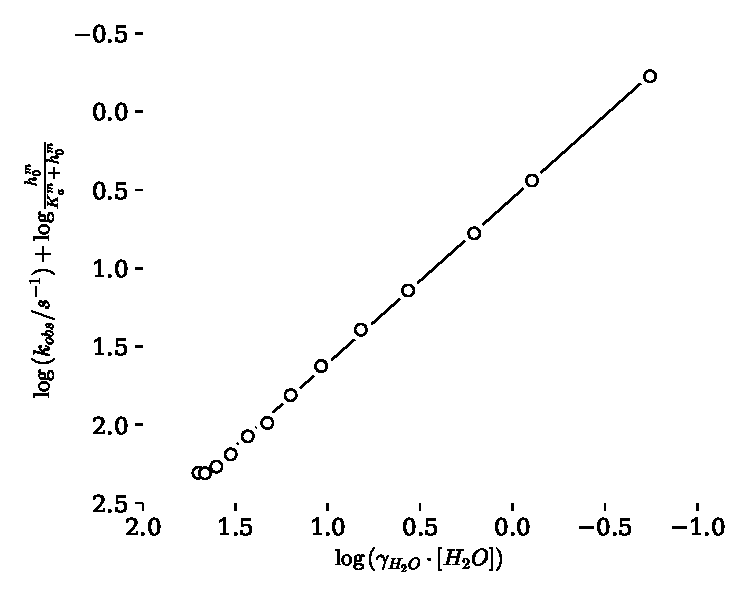
\includegraphics[scale=0.7]{images/fig18}
  \label{fig:fig18}
\end{figure}


\begin{marginfigure}[-40mm]
  \centering
  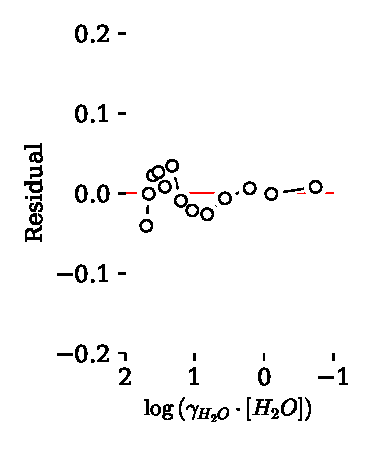
\includegraphics[scale=0.7]{images/fig18r}
  \caption{A plot of the residuals. $\uparrow$} 
  \label{fig:fig19}
\end{marginfigure}

We need an anchor. The authors proposed that the acidity function for esters in sulphuric acid mixtures would be $0.62H_0$. However they also reported that others had pegged it at $0.65H_0$.  There appears to be wiggle-room there. The $pK_a$ value for protonated aliphatic esters are estimated to be in the range of $-7$ to $-8$. The value for $pK_a$ determined from the optimization in figure~\ref{fig:fig15} was well away from those values. Let us compromise on a value for $pK_a$ and set it to $-7.5$ and the optimize the value of $m$ to achieve the best linear fit.

\subsection{Optimizing for $m$ with $pK_a = -7.5$}

\begin{marginfigure}[20mm]
  \centering
  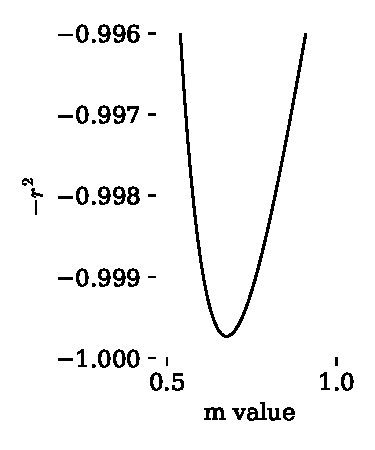
\includegraphics[scale=0.7]{images/fig20}
  \caption{A plot of $r^2$ as $m$ is varied with $pK_a = -7.5$ . The best fit occurs at $m = 0.68$. $\uparrow$  \\ \vspace{3mm} The \textit{Python} notebook for the plots in Figures~\ref{fig:fig18}, \ref{fig:fig19} and \ref{fig:fig20} above can accessed via Google Colab at \url{https://colab.research.google.com/github/blinkletter/4410PythonNotebooks/blob/main/Class_30/Yates-Fig15-rate_vs_aH2O.ipynb} and setting the variables of $pK_a$ and $m$ accordingly.} 
  \label{fig:fig20}
\end{marginfigure}

We can vary the value of $m$ while holding $pK_a = -7.5$ and we see that the optimal value for $m$ is 0.676. This is very close to the reported observations of Lane\textsuperscript{\ref{ref:ref6}} and Yates.\textsuperscript{\ref{ref:ref1}} In figure~\vref{fig:fig21} we again plot $\log{k_{obs}}-\log{\frac{h_0^m}{K_a^m + h_0^m}}$ vs. $\gamma_{\ce{H2O}} \cdot [\ce{H2O}]$ using these parameters and we again get an excellent plot. The plot of the residuals in figure~\ref{fig:fig22} shows a more random distribution. However, if you examine the residual plots so far you may have noticed that the point at the highest concentration of \ce{H2SO4} (the lowest value for $a_{\ce{H2O}}$) seems to have the largest residual when using $pK_a$ values closer to observations. This point is out at the start of an inflection in the rate curve (see figure~1 of the paper.\textsuperscript{\ref{ref:ref1}})

\begin{figure}[h!]
  \centering
  \caption[][-0mm]{Plot of $\log{k_{obs}}-\log{\frac{h_0^m}{K_a^m + h_0^m}}$ vs. $\gamma_{\ce{H2O}} \cdot [\ce{H2O}]$ where $m = 0.68$ and $pK_a = -7.5$. \\ $\longleftarrow$ \\ The line equation is\ldots \begin{align*}y &= 1.84x+1.50 \\ r^2 &= 0.999\end{align*}} 
  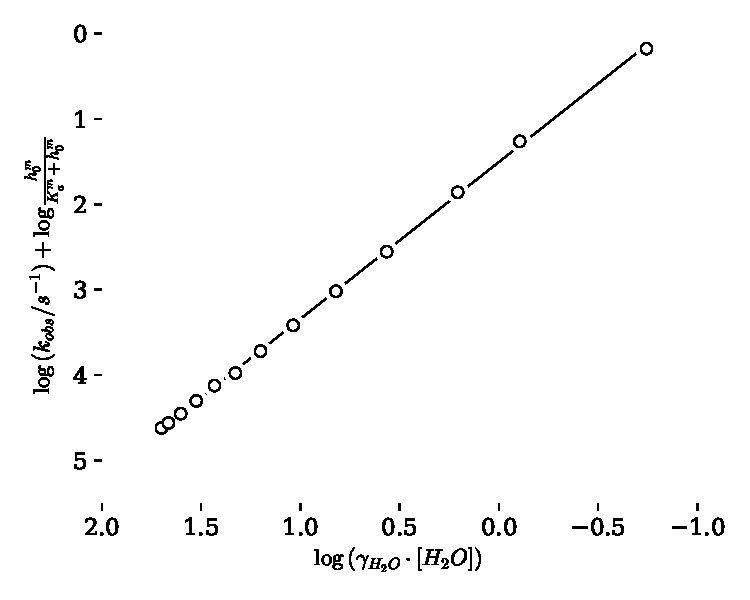
\includegraphics[scale=0.7]{images/fig21}
  \label{fig:fig21}
\end{figure}


\begin{marginfigure}[-40mm]
  \centering
  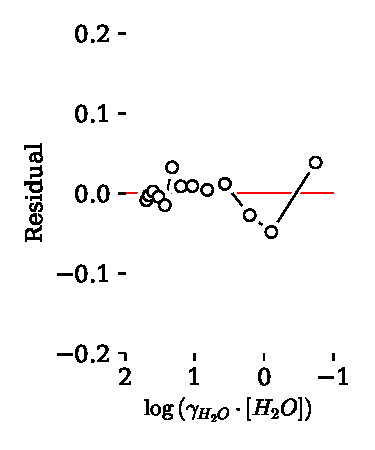
\includegraphics[scale=0.7]{images/fig21r}
  \caption{A plot of the residuals. $\uparrow$  \\ \vspace{3mm} The \textit{Python} notebook for the plots in Figures~\ref{fig:fig21} and \ref{fig:fig22} above can accessed via Google Colab at \url{https://colab.research.google.com/github/blinkletter/4410PythonNotebooks/blob/main/Class_30/Yates-Fig20-rate_vs_aH2O.ipynb}} 
  \label{fig:fig22}
\end{marginfigure}





\subsection{Getting Picky About a Point}

Perhaps the point at highest $\% \ce{H2SO4}$ is starting to include a significant amount of the other hydrolysis mechanism that becomes predominant at extreme acid mixtures. The authors do not include it in the line fit for their own determination of the slope when they plotted $\log{k_{obs}}+m H_0$ vs. $\log{a_{\ce{H2O}}}$ in figure~3 of the paper.  

The slight deviation in rate is not great enough to exclude it from the data set using standard statistical tests but, since we see a curve in the plot in figure~3 of the paper, we might use our chemical instinct to justify excluding this last point on the journey to the other mechanism from the data set for the $A_{Ac}2$ mechanism.

We will remove the last data point in table~\vref{tab:tab1} and perform an uncontrained optimization of both $m$ and $pK_a$. The results are displayed in figures~\ref{fig:fig24}, \ref{fig:fig25}, and \vref{fig:fig23}.


We see in figure~\ref{fig:fig23} that the best fit occurs at $m = 0.69$ and $pK_a = -7.0$. These values are very close to what the authors report from ex\-per\-imental observations. However they must be taken with a grain of salt given the very flat surface of the optimization. The fact that they agree with experiment is very encouraging.


\begin{figure}[h!]
  \centering
  \caption[][-0mm]{Plot of $\log{k_{obs}}-\log{\frac{h_0^m}{K_a^m + h_0^m}}$ vs. $\gamma_{\ce{H2O}} \cdot [\ce{H2O}]$ where $m = 0.69$ and $pK_a = -7.0$. The highest \%\ce{H2SO4} point that was excluded is shown in red.\\ $\longleftarrow$ \\ The line equation is\ldots \begin{align*}y &= 1.88x+1.19 \\ r^2 &= 0.9999\end{align*}} 
  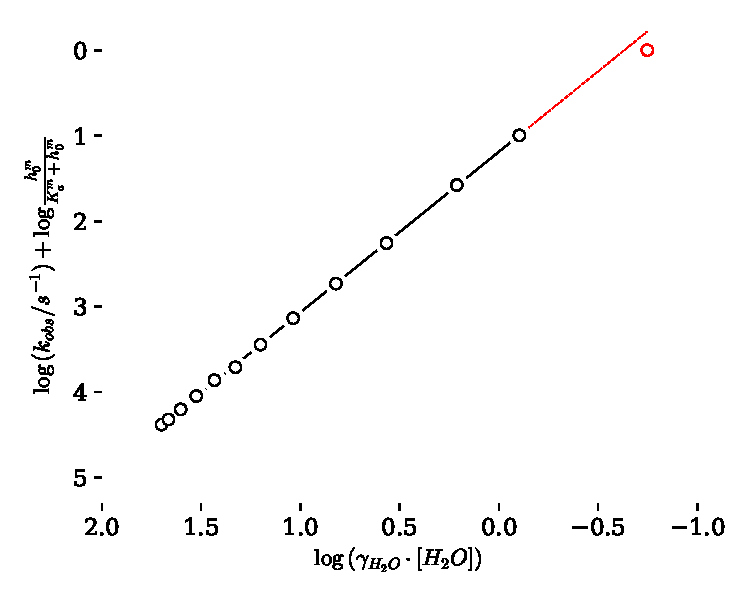
\includegraphics[scale=0.7]{images/fig24}
  \label{fig:fig24}
\end{figure}


\begin{marginfigure}[-40mm]
  \centering
  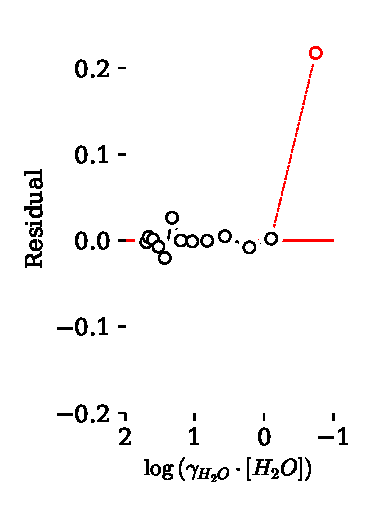
\includegraphics[scale=0.7]{images/fig24r}
  \caption{A plot of the residuals. The highest \%\ce{H2SO4} point that was excluded is shown in red. $\uparrow$} 
  \label{fig:fig25}
\end{marginfigure}

When I plot $\log{k_{obs}}-\log{\frac{h_0^m}{K_a^m + h_0^m}}$ vs. $\gamma_{\ce{H2O}} \cdot [\ce{H2O}]$ with $m = 0.69$ and $pK_a = -7.0$ in figure~\ref{fig:fig24}, I see another high quality fit with very small and apparently random residuals as shown in figure~\ref{fig:fig25}. The order of reaction in $[\ce{H2O}]$ is shown to be 2 with the observation of a slope of 1.9 in the plot.

\begin{marginfigure}[0mm]
  \centering
  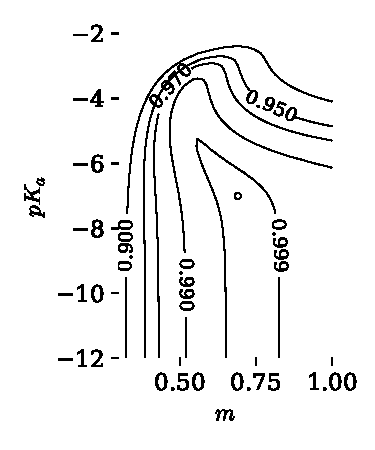
\includegraphics[scale=0.7]{images/fig23}
  \caption{A contour plot of the surface for $r^2$ as $m$ and $pK_a$ are surveyed when the highest \%\ce{H2SO4} point that was excluded. The best fit occurs at $m = 0.69$ and $pK_a = -7.0$ although the surface is very flat for a broad area around those values. $\uparrow$ \\ \vspace{3mm} The \textit{Python} notebook for the plots in Figures~\ref{fig:fig24}, \ref{fig:fig25} and \ref{fig:fig23} above can accessed via Google Colab at \url{https://colab.research.google.com/github/blinkletter/4410PythonNotebooks/blob/main/Class_30/Yates-Fig23-rate_vs_aH2O.ipynb}} 
  \label{fig:fig23}
\end{marginfigure}

\section{Conclusion}

I disagreed with the authors choice of independent variable for their kinetic analysis. The water activity as reported by Giauque et al.\textsuperscript{\ref{ref:ref2}} was a mole fraction and not a molar quantity. However the conversion to effective concentration of water made very little difference. It is still the better way to plot the results in my opinion. The authors used experimental observations to establish an acidity function ($0.62H_0$) and a $pK_a$ value of $-7.2$ for the protonated aliphatic ester. These values gave a slope very near a value of 2 and indicated that the molecularity of water in the r.d.s. is two.

I deleted the single point at highest acidity in the data that was at the beginning of the transition to the other mechanism and, when I optimized the values for the acidity function and the $pK_a$ value without constraints, the values for the acidity function and $pK_a$ for esters was found to be $0.69H_0$ and $-7.0$, respectively. The slope was again very near a value of 2. 

We have examined and recalculated the results of Yates et al. and, although we used slightly different methods, obtained exactly the same conclusions the authors. Nothing changed --- time well spent.

Now use these methods to replot all the data sets in the paper\textsuperscript{\ref{ref:ref2}} and confirm that we can get very similar results for the $A_{Ac}2$ mechanism using their data and our own approach.


\end{document}
